\chapter{Introduction}
This thesis aims to explore emotion recognition and its effectiveness in the Swedish language. With the rapid advancement of the technology industry and artificial intelligence, emotion recognition has started to play an increasingly important role in the enhancement of human-computer interactions. These areas hold potential to transform and develop several important fields, but there are still challenges in the field. Much of the research has been focused on specific languages, notably English. This research focuses on emotion recognition across two distinct modalities in Swedish, speech-based emotion recognition and text-based emotion recognition and aim to contribute to broadening the field of emotion recognition in a non-English language.

\section{Background}
Emotion recognition has attracted increasing attention with the rapid advancement of technology and artificial intelligence. Emotions are experienced by all humans but are difficult to define precisely. They are an internal experience that are foundational to our sense of identity, our relationships, and moral judgement. Scientists have faced challenges in the effort to characterize how emotions are communicated. Emotions are internal but also expressed externally through voice and movements of the body. They are not only communicated through the words we say, but also how we say them. Tones of the voice is a source of varied emotional expressions where its states may alter patterns in vocalizations. It is considered that various emotion-related physiological changes influence acoustic features such as pitch, tempo, pitch variability, and loudness in the speech \autocite{Oatley2019}.
Scientists have developed different techniques to determine states of emotions as well as opinions, a field of Natural Language Processing (NLP) that intersects artificial intelligence, computer science, and linguistics \autocite{Kansara2020}. With the development of Artificial Intelligence several techniques have accelerated in the recent years, including for NLP, even if its origins back to the 1950s when questions about whether a machine could learn and think to interact with humans \autocite{Alvarez2024}. NLP has remained as a significant contributor of AI. Some of the active research areas in the NLP domain is Machine Translation, Chatbots, recognizing speech, text summarization, and sentiment analysis \autocite{Kusal2023}. Figure \ref{fig:subdomains-AI} demonstrates the different subdomains of AI. 

\begin{figure}[ht]
    \centering
    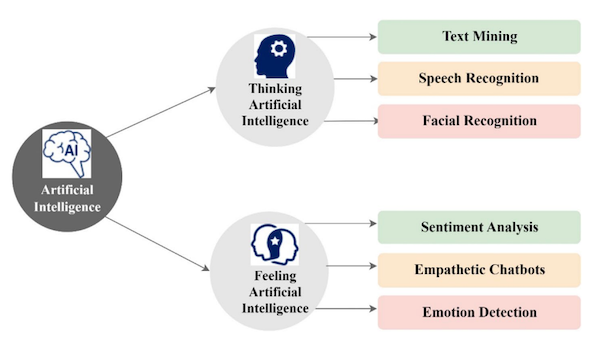
\includegraphics[height=7cm]{png/subdomains AI.png}
    \caption{\textit{Subdomains of AI \autocite{Kusal2023}}.}
    \label{fig:subdomains-AI}
\end{figure}

Sentiment analysis is a computational branch in NLP that utilizes the detection and evaluation of people’s emotions, opinions, and moods based on text, speech, facial expression, etc., without analyzing these feelings \autocite{Ermakova2023}. The rise of sentiment analysis is associated with the growth of social media, which has generated vast amounts of digital option data recorded in digital forms. Since the early 2000’s, the field has become one of the most researched parts in NLP \autocite{Zhang2018}, expanding beyond computer science to fields like finance, marketing, political- and health science. Accordingly, sentiment analysis is valuable across different areas of society. Sentiment analysis is utilized in the popular index called the happy planet index \autocite{HappyPlanetIndex}, measuring sustainable well-being of different countries, even if it only can observe three feelings, positive, negative, or neutral. The happy planet index checks the happiness level calculated from a particular country, where emotion detection is used with sentiment analysis \autocite{Madhuri2021}.
With the evolution of deep learning networks, emotion detection has advanced. Sentiment analysis identifying positive, negative, or neutral states have progressed into recognizing the six basic emotions; joy, sadness, anger, disgust, fear, and surprise in text \autocite{Safari2023}. The emotions categorization fluctuate depending on the research. These basic six where determined by Paul Ekman \autocite{Oatley2019, Kusal2023} who determined that these six fundamental emotions is shared in people of different cultures, characterized by facial features. However, Ekman’s classification was made over 20 years ago when no agreement about what emotions should be considered as existed. Today, the agreement about evidence for universal emotional signals and evidence for five emotions is robust: anger, disgust, sadness, happiness, and fear \autocite{Ekman2016}.

Emotion recognition is accomplished either through text or speech, with numerous studies in both areas. Text-based emotion detection is a complex field that requires a very clear understanding of the context. Today this technique is frequent in several fields, such as human-computer interaction, big data, data mining, e-commerce, online tutorials and psychology \autocite{Madhuri2021}. The first emotion dataset, The International Survey on Emotion Antecedents and Reactions (ISEAR) was developed in 1997, after it was stated that computers need the ability to interpret, express, and identify emotions if we want true intelligent computers and be able to communicate with them naturally \autocite{Kusal2023}.

Emotion recognition from textual data is important in various domains such as customer reviews, social media analysis, public monitoring, and conversational agents. A systematic review \autocite{Kusal2023} shows that Deep Learning models outperform traditional Machine Learning models due to their ability to capture contextual dependencies. The review further demonstrates the highest accuracy is shown by transformer-based models such as bidirectional encoder representations from transformers (BERT), highlights challenges such as small or imbalanced datasets that can affect the model reliability, and notes that multimodal approaches with text, speech, and images improve emotion recognition. BERT-technology is leveraged with a model that outperformed other text-based emotion recognition models, with 76\% validation accuracy \autocite{Madhuri2021}. However, text-based emotion detection (TBED) has challenges with identifying hidden emotions, and adapting to diverse languages. Datasets based on different languages than English, as Arabic and Hindi, are tested in a study \autocite{Maruf2024} that identifies challenges as limited resources for non-English languages. The authors underscore the potential of TBED but notes limitations as it is no universal solution for challenges like sarcasm, dynamic emotions, and cultural variances.

Emotion detection research progressed with Speech Emotion Recognition (SER) \autocite{Kusal2023}. It has shown that hearers can evaluate five emotions in speech-prosody, anger, happiness, sadness, fear, and tenderness, with 70 percent accuracy \autocite{Oatley2019}. Speech emotion recognition focuses on how something is said rather than the words themselves. Acoustic features like amplitude, formants, and pitch help classify emotions. A common approach uses Mel-frequency cepstral coefficients (MFCCs), which capture vocal patterns and have proven effective in detecting emotions \autocite{Thaler2024}. Those features offer invaluable insights into the subtle emotional expressions conveyed through speech, assisting the complicated process of emotion recognition. They are typically categorized into three primary groups: prosodic features, voice quality features, and spectral features \autocite{Lian2023}.

Several studies distinguish different emotions through vocal features. Already in 2005, Lee \& Narayanan investigated automatic recognition of emotions, especially positive vs. negative from spoken dialogs. In that study, acoustic, lexical, and discourse information were combined to enhance emotion detection and move beyond traditional acoustic-only ways. The authors analyzed acoustic features, lexical features, and discourse features. Linear Discriminant Classifiers were used and resulted in good performance for acoustic and lexical information \autocite{ChulMinLee2005}. In 2014, one study \autocite{Bnziger2014} showed that regular people can rate how voices sound reliably, when actors pretend to feel emotions, sometimes better than machine sound measurements for pitch and volume. The human voice feature rating worked better than technical measures, especially for happy emotions. 
These acoustic features in our voice enable emotion recognition through speech using Deep Learning, which have many advantages for Speech Emotion Recognition over traditional sentiment methods. Deep Learning has the capability to detect complex structures and different features without requiring manual feature extraction \autocite{Khalil2019}. SER’s goal is identification of emotions in speech, unrelated to the semantic content \autocite{Kusal2024}. Figure \ref{fig:blockdiagram-SER} represents a SER system. 

\begin{figure}[ht]
    \centering
    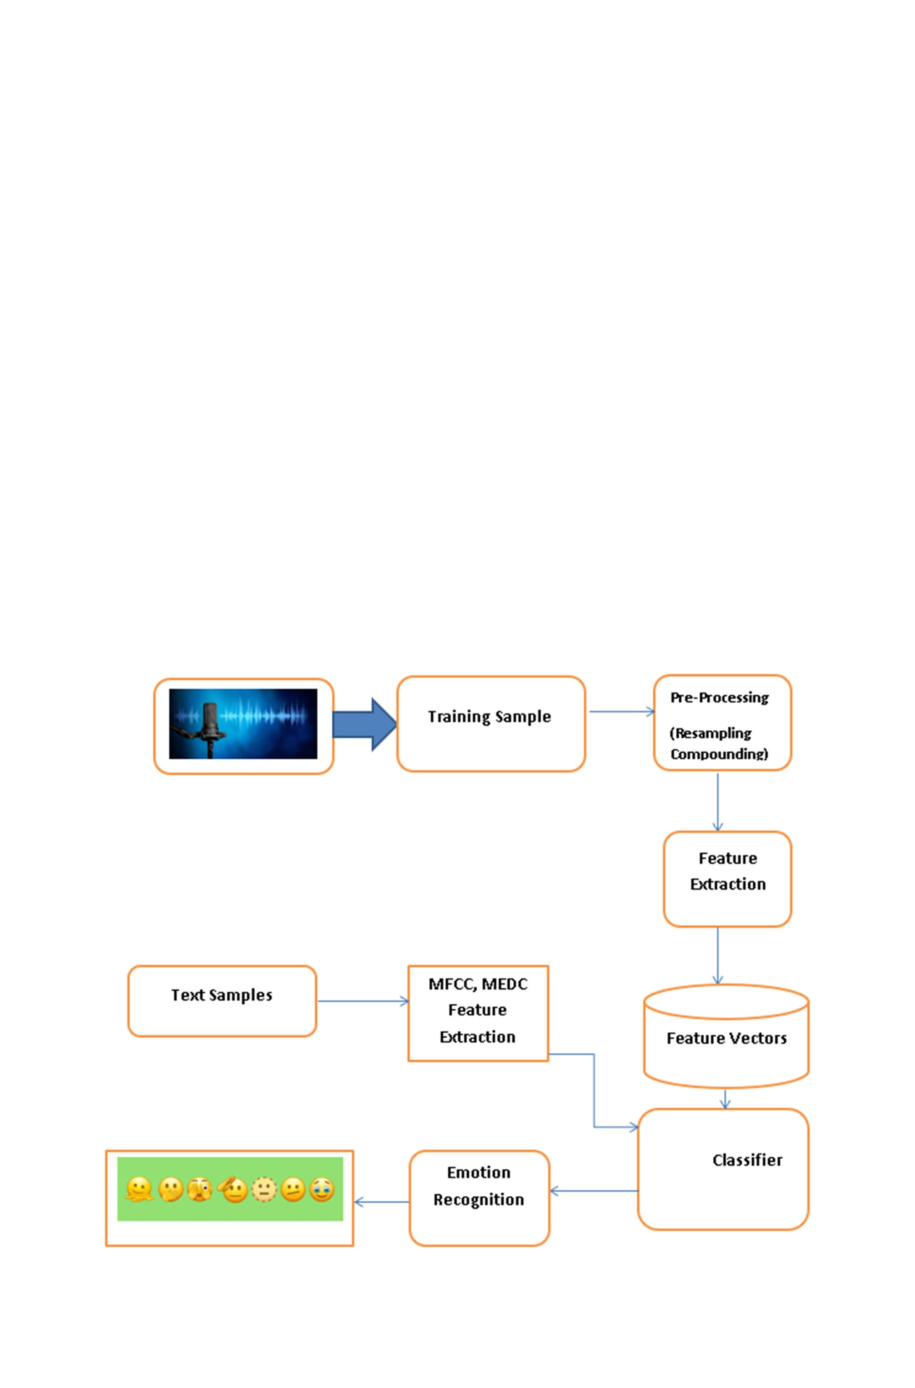
\includegraphics[height=7cm]{png/background/block-diagram.pdf}
    \caption{\textit{Block diagram of SER \autocite{Tyagi2024}.}}
    \label{fig:blockdiagram-SER}
\end{figure}

In recent years, speech emotion recognition has emerged as a significant and complex research area within pattern recognition, speech signal processing, and artificial intelligence. Its growing importance is driven by its applications in human-computer interaction. Specifically, SER systems enable emotion-aware interactions through speech, eliminating the need for traditional input devices. This advancement has led to the development of intelligent affective services in fields such as call centers, healthcare, surveillance, and affective computing \autocite{Zhang2021}. The accuracy of models tested in recent years have improved significantly. Several studies conducted in the last year’s show emotion detection accuracy results over 90\% \autocite{Adebiyi2024, Praseetha2022, Rahman2024}. A research paper \autocite{Abbaschian2021} compares several studies, detailing the results, databases used, and the time periods during which the studies were conducted. The reported accuracies depends greatly on which model was used, as well as the tested dataset. According to Abbaschian (2021), in 2014, one model showed 54.3\% accuracy for the IEMOCAP dataset. The same dataset was used for the LSTM model in 2017 and 2018 with 63.5\% respectively 64.93\% accuracy. When the same dataset was tested with a CNN-model, the accuracy increased to 82.8\% in 2019.  

A study \autocite{Juslin2018} concluded in 2018 analyzed 1,877 voice clips from 23 datasets to compare spontaneous and posed emotions. Their findings highlighted key differences: 
\begin{itemize}
    \item Spontaneous expressions were rated as more genuine than posed ones, even when intensity was controlled. 
    \item Posed expressions were more intense, but intensity alone did not fully explain perceived authenticity. 
    \item Acoustic differences were small but present, mainly in pitch range, speech rate, and voice intensity. 
    \item Highly intense spontaneous emotions conveyed emotions as clearly as posed ones, suggesting that emotion intensity plays a role in perception. 
\end{itemize}
These findings suggest that posed and spontaneous emotions are not interchangeable and that datasets used in SER research must account for these differences to ensure reliable models. 

One study \autocite{Rathi2024} presents a comprehensive review of SER which explores the impact of speech data corpora selection and speech feature extraction on the accuracy of emotion classification. Publicly available speech datasets from 2014-2023 are systematically analyzed and categorize speech datasets and speech features to evaluate their impact on the accuracy of emotion recognition. The study by Rathi \& Tripathy (2024) includes the six emotions: happiness, anger, sadness, surprise, fear, and neutrality. According to Scherer, Frühholz \& Belin (2018), most studies focus on only four broad emotion categories: anger, fear, happiness, and sadness, which is seen as a limitation by the authors \autocite{Scherer2018}. However, emotion classification fluctuates in different studies. A database has been conducted that unravel this limitation. The database is called GoEmotions \autocite{Demszky2020} which is a big, detailed, and reliable dataset for recognizing 27 emotions in text. The researchers \autocite{Demszky2020} used a BERT model and got an average F1-score of 0.46 for these emotions, best for gratitude (0.86) and worst for grief (0.00). The model performed a score of 0.64 for the simpler 6 emotion grouping. The authors conclude that the model still needs advancements for tricky feelings but suggest the model as a good starting point. This research is included in the research that the AI-model Hume.ai builds upon \autocite{HumeAI-AboutHume}, which is important to acknowledge since it might affect biases. Most researchers focus on the fundamental and widely recognized emotions. The six fundamental emotion model by Paul Ekman is the most widely used for both text-based and speech-based emotion recognition \autocite{Maruf2024}.

Datasets are essential for data-driven learning, enhancing model performance and robustness. Emotion recognition datasets are classified based on signal type, including speech (textual/audio), visual, physiological signals, and multimodal data. Speech emotion datasets are further classified by how they are collected: 
\begin{itemize}
    \item Performer-based datasets feature emotions acted by trained performers. 
    \item Induced datasets capture emotions in controlled environments, making them less expressive but closer to real-life emotions. 
    \item Natural datasets come from real conversations (e.g., public dialogues, call centers) and contain authentic emotional variations but are more challenging due to background noise and limited availability \autocite{Cai2023}. 
\end{itemize}
Most research in the field of SER investigates the accuracy of different Deep Learning algorithms on diverse public datasets. A review \autocite{Rathi2024} analyses 93 research papers where IEMOCAP and RAVDESS are among the most widely used datasets, chosen by 35.83\% and 21.50\% of researchers, respectively. Their popularity stems from well-annotated data and diverse range of emotional expressions, which enhance model performance. Figure \ref{fig:datasets-percentage} presents the usage of the datasets in this review.  
\begin{figure}[ht]
    \centering
    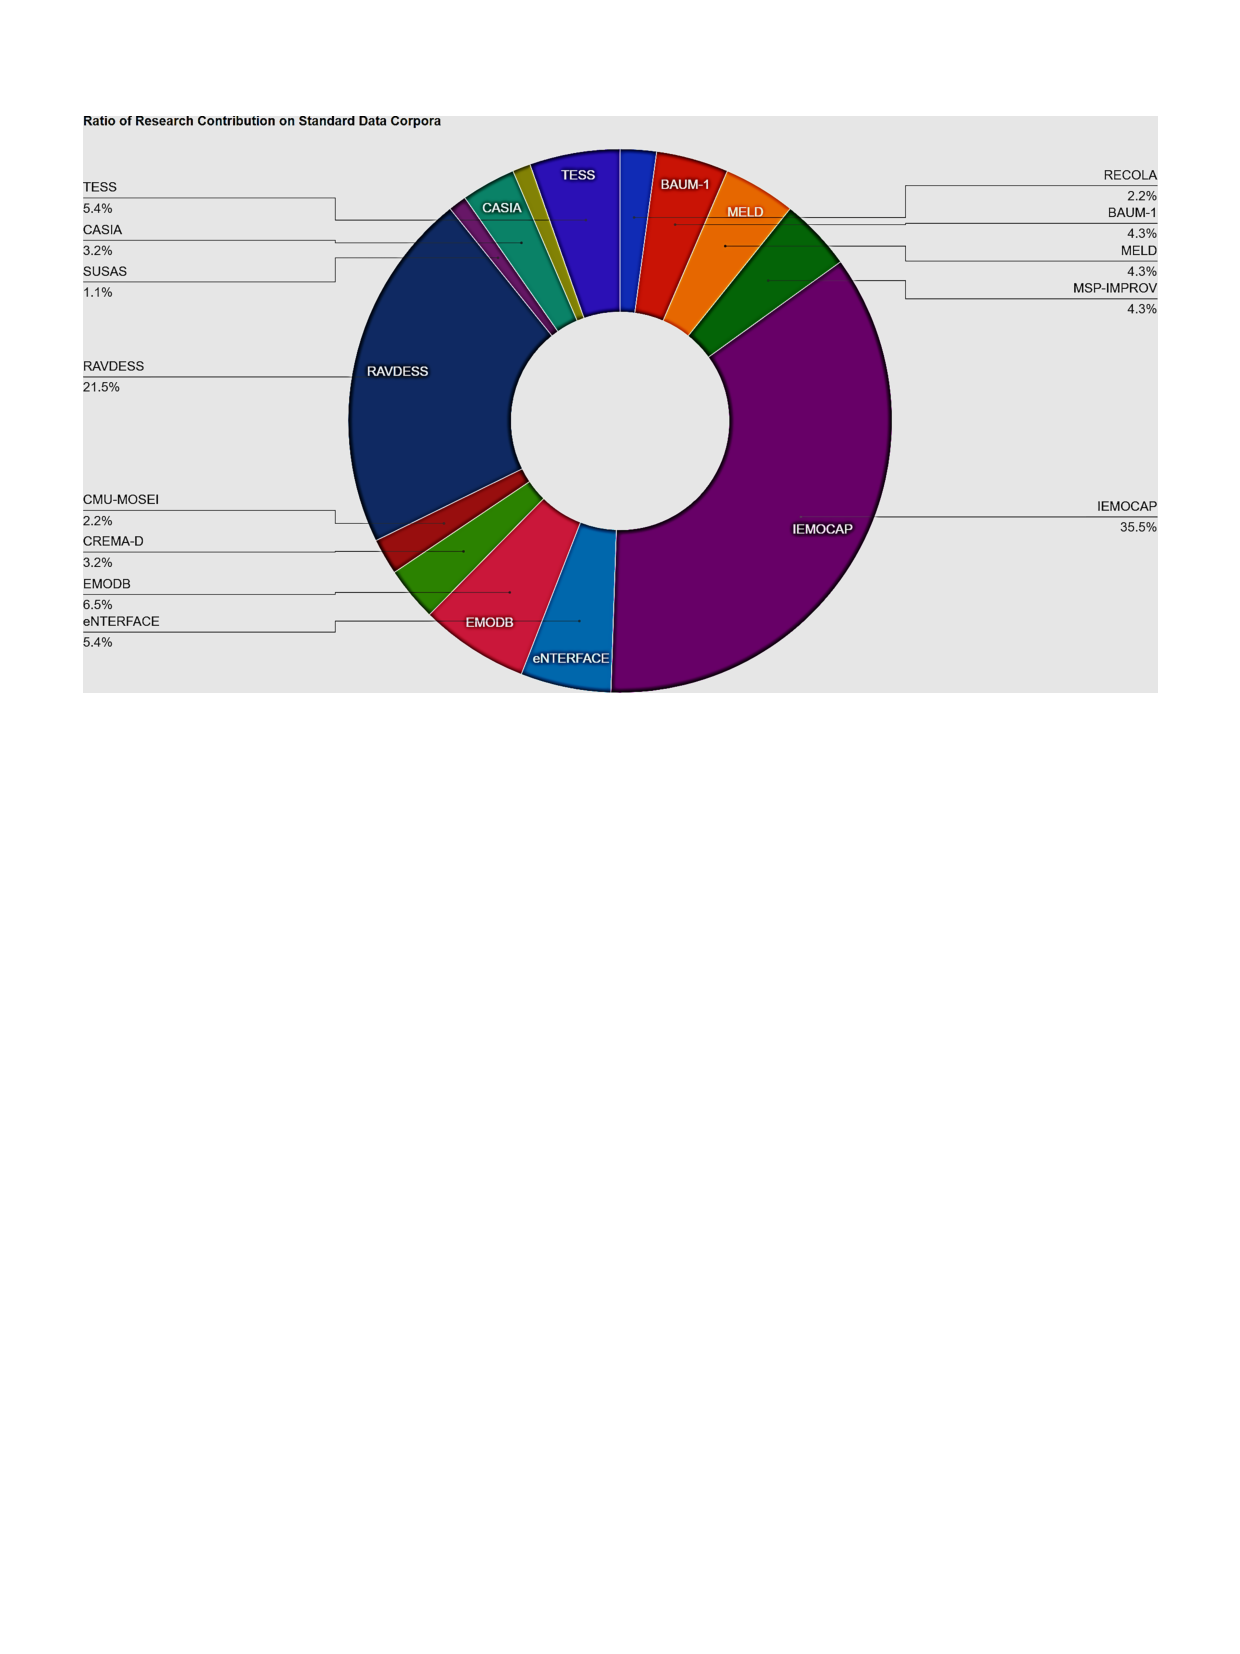
\includegraphics[height=8cm]{png/background/datasets-diagram.pdf}
    \caption{\textit{Research contributions of standard data corpora in percentage}\autocite{Rathi2024}.}
    \label{fig:datasets-percentage}
\end{figure}
The paper \autocite{Rathi2024} includes varying datasets in terms of linguistic diversity, recording conditions (acted, induced, or natural speech), and the number of emotional categories. The results show that the choice of dataset significantly affects the model's performance. Key features such as Mel-Frequency Cepstral Coefficients (MFCCs), pitch, intensity, prosodic cues, and spectral properties impact SER accuracy significantly. The authors discuss the balance between realistic datasets and classification accuracy, noting that natural speech is more difficult to classify due to its high variability and noise in natural speech. 

The number of natural datasets is relatively limited \autocite{Cai2023}, and many research papers test on acted datasets. An empirical analysis \autocite{Ahammed2024} of Machine Learning algorithms across diverse datasets, concluded in 2024, demonstrates high-accuracy SER system using an SVM classifier and advanced feature extraction techniques. The model performed exceptionally well across multiple datasets (RAVDESS, TESS, SAVEEE, and combined dataset), with the combined dataset achieving perfect scores (100\%) in accuracy, precision, and F1-score. Two of these datasets, RAVDESS \autocite{StevenRLivingstone2019} and TESS \autocite{Pichora-Fuller2020}, are acted and the SAVEE \autocite{kaggle-savee} dataset was recorded from four male, postgraduate students and researchers. All three datasets are in recorded in English. 
The TESS dataset was used in a study from 2022 \autocite{Praseetha2022} that leveraged other techniques, with one original dataset and one augmented dataset. Achieved accuracy was 93\% and 97\% for the augmented dataset, resulting in a significant improvement for the processed data.
A different study \autocite{Alroobaea2024} from 2024 investigates transformers for SER in cross-corpus scenarios. The recordings are preprocessed to remove noise, and augmented techniques are applied. Three datasets were used, two the same as the previous study, SAVEE and RAVDESS, with the Berlin Database of Emotional Speech, Berlin EMO-DB, including ten professional speakers, was additional. A combined cross-corpus dataset of the three sets were used to test generalizability across different datasets. This proposed transformer-based model outperformed traditional deep learning methods. The model showed high accuracy results with 95\% for SAVEE, 94\% for RAVDESS, 97\% for EMO-DB, and 97\% for the cross-corpus dataset. However, this model was not evaluated on spontaneous speech datasets.
Comparing these three studies from 2022 to 2024 reveals a clear trend of increasing accuracy over time. A 2019 review \autocite{Khalil2019} reported significantly lower results for the SVM, with accuracy of 74\% for anger, 70\% for happiness, and 93\% for sadness. However, the same study found that a Deep Convolutional neural network (DCNN), achieved substantially higher accuracy, with 99\% for both anger and happiness, and 96\% for sadness. Both Emo-DB and SAVEE datasets were included, as well as IEMOCAP which also is an acted dataset recorded in English.

Datasets for Text Based Emotion Detection (TBED) are discussed in \autocite{Kusal2023}, where the authors state that researchers can use publicly available datasets or create their own. Publicly available, useful datasets with reliable annotating include several sets based on various data, from stories, publications, news, social media texts, to reviews on movies. The datasets emotion-classification reaches from the basic six emotions to GoEmotions set that include 27 emotions. Many datasets are based on social media, including casual writing style which is a big challenge. The use of short messages and informal language has limited research. Human emotion expressions and the texts conveying them are ambiguous and subjective, additionally, emotions are multifaceted with varying expressions. Therefore, the authors claim that human mapping is important. 
Self-labeled emotion datasets are tested in a study \autocite{Lee2023} that uses a Transformer Transfer Learning (TTL) model trained on a dataset of over 3.5 million tweets with self-reported emotion hashtags. The model is tested against 10 prior published datasets and achieved highest score on annotator-rated sets (0.87), it also performed well on self-reported sets (0.79) which demonstrates generalizability.  

The promising development of emotion recognition has been adapted in research for other areas than computer and machine learning science. SER is beneficial in translating languages, interactive courses and tutorials held online where the student’s emotional state can be understood to help the machine make decisions on how to present the course. It can be implemented in vehicles’ safety structures to recognize the driver’s emotional state and therefore prevent accidents \autocite{Abbaschian2021}. The mental health sector has great potential to benefit from emotion recognition. Several studies \autocite{DeSouza2021, Drougkas2024, Simcock2020,Singh2023} have investigated how AI-based emotion recognition can be used to help therapists and psychiatrics diagnosing and identifying potential mental illnesses. One of the studies \autocite{DeSouza2021} demonstrates how leveraging speech and text analysis with NLP can help detect late-life depression. It showed consistent alterations in individuals with depression, including acoustic features such as pitch, speech rate, pause duration, and word choice. The authors suggest that automated speech analysis can identify late-life depression as well as predicting depression severity with accuracy of 86-92\%. Multimodal machine learning with a combination of text and audio analysis has been explored to identify indicators for various mental health disorders. The research \autocite{Drougkas2024} compared unimodal text models, which showed strong results but was outperformed by the multimodal models, especially for identification of the presence of markers. The multimodal models achieved accuracy up to 86.73\%. This study highlights the importance of machine learning integration in mental health diagnostics. 

\section{Problem Description}
Despite significant progress in speech emotion recognition, there are limitations in current research. For instance, emotional voice samples are usually obtained from actors portraying emotions using scripted speech. These acted expressions tend to be more intense and exaggerated than naturally occurring emotions. However, this method risks overemphasizing obvious emotional cues while missing subtle ones. It is argued that such portrayals reflect social norms more than genuine physiological responses, although all public expressions may involve some degree of performance \autocite{Scherer2018}.

The way emotional speech data is collected depends on the design and purpose of the SER system. As datasets shift from acted emotions to more spontaneous or real-life emotions, emotion recognition becomes more challenging. Many researchers prefer acted emotion datasets because they offer a wide range of emotions and large amounts of data \autocite{Rathi2024}. Induced datasets are collected by constructing an artificial emotional situation, without the knowledge of the performer or speaker. This results in a more naturalistic database, but issues regarding ethics may apply, since the speaker should know they have been recorded for research \autocite{Khalil2019}. 

Estimation of emotions from spontaneous speech is a challenging task. Most studies test models on acted datasets \autocite{Khalil2019, Ahammed2024, Praseetha2022, Alroobaea2024}. The primary reason for the concentration on acted SER tasks is that acted emotions can be easily performed in a controlled laboratory setting, often resulting in high SER accuracy. However, these emotions tend to be exaggerated and may not accurately reflect how emotions are expressed in real-world situations. Consequently, detecting spontaneous emotions in natural environments is significantly more complex and challenging compared to recognizing acted emotions \autocite{Zhang2021}. Figure \ref{fig:databases-diff} demonstrates the difficulty level for varying settings.

\begin{figure}[ht]
    \centering
    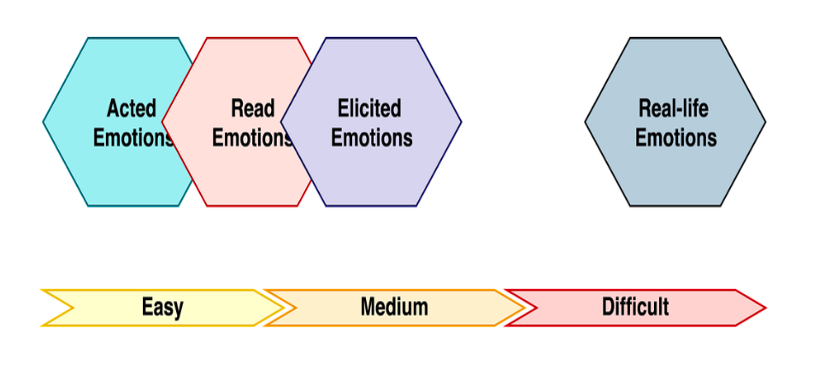
\includegraphics[height=6cm]{png/databases difficulty.png}
    \caption{\textit{Emotion recognition databases and their difficulty level \autocite{Khalil2019}.}}
    \label{fig:databases-diff}
\end{figure}
One study from 2019 \autocite{Milner2019} using four English speech datasets, two acted (eNTERFACE and RAVEDESS), one elicited (IEMOCAP), and one natural (MOSEI), to see how emotions can be recognized across them. The researchers in this study tested different training methods to explore whether mixing acted and natural data works. They found that acted data does not easily help with natural emotions unless the system is tweaked. The differences in real and acted voices are shown in other studies as well \autocite{Juslin2018}. Real ones sound more genuine and have some unique features, even if the basic emotion patterns are alike. When emotions are strong, real voices can show clear emotions just as well as acted ones, which supports an idea that strength matters more than whether it is real or fake.

Speech emotion recognition (SER) plays a crucial role in identifying emotions from speech. However, because emotions are complex and often overlap, extracting accurate emotional features from speech remains challenging. As SER research advances, cross-cultural emotion recognition is becoming increasingly important. While people from different countries and cultures have distinct ways of expressing emotions, they can still interpret tone and attitude even without understanding the spoken language \autocite{Cai2023}. Behind the development of the SER model Hume.ai, a study \autocite{Brooks2023} on cultural differences in vocal bursts has been conducted. It is suggested that 24 acoustic dimensions of vocal expression have emotion-related meanings that distinguish them. With participants from China, South Africa, Venezuela, India, and the USA, the authors concluded that 79\% of complex vocal modulations were preserved across these countries. Research shows that speech acoustics change based on emotion, intensity, and cultural background. Studies comparing tonal and non-tonal languages \autocite{Scherer2018} suggest that features like pitch and speech rate are influenced not only by physiology but also by cultural differences in emotional expression. It is debated whether emotional expressions are universal or culturally influenced is particularly relevant to vocal emotion recognition, as languages differ in phonemic structure, intonation, and rhythm. If emotion expression differs between languages, emotion recognition across cultures may also be affected. One study from 2001 is referred in \autocite{Scherer2018}, where listeners from seven countries recognized emotions in German-accented speech. While accuracy averaged 66\%, recognition rates varied significantly, from 74\% in Germany to 52\% in Indonesia, indicating that cultural and linguistic differences impact vocal emotion perception. 

The Swedish language is not widely spoken and therefore very limited research has been concluded on the Swedish speech. One study \autocite{Ekberg2023} investigated Swedish emotion recognition through feature extraction and concluded that emotions in Swedish speech have unique sound patterns. The results from this study differed from previous research in some spots, which could be due to the language itself. The emotion results showed that surprise is a very distinct emotion, but happiness and anger sound alike, which could confuse listeners. 

There are studies that explore SER for different languages. EMO-DB is a Berlin Database of Emotional Speech that is used in several studies with high accuracy \autocite{Alroobaea2024, Khalil2019, Zhao2019, Jahangir2022}. SER across different cultures and languages are explored in an article \autocite{Pandey2023} that tackles the challenge of recognizing emotions in speech from five languages: English, German, Persian, Hindi, and Telugu, since emotions can sound different depending on the speaker and language. A language model was pre-trained on four languages to identify language-specific cues and applied to the remaining one, Persian. Two different methods were tested, one excelled with known languages (92.24\% unweighted accuracy for English), and resulted in 63.09\% unweighted accuracy for the new language. The second method had similar results, with up to 95\% accuracy for pre-defined language but struggled with unseen languages. Emotional variation due to culture and speech is mentioned in this study as well, for example, Hindi anger might sound different than German anger. 

Similarities as well as differences in cultural and linguistical vocal features affecting emotions are declared depending on the research. Studies using common databases on other languages than English, such as the German EMO-DB \autocite{Alroobaea2024, Khalil2019, Zhao2019, Jahangir2022}, cannot generalize linguistic performance since many of the models in these studies are trained on these databases. The studies highlight that models trained on specific databases like the Berlin EMO-DB or pre-trained on a limited set of languages struggle to achieve high accuracy when applied to unseen languages, such as Persian, due to cultural and linguistic variations in emotional expression. Therefore, these models cannot be considered as generalizable to other languages, as their performance is dependent on the linguistic and cultural conditions of the data it was trained on. 

\newpage
\section{Purpose and Research Questions}

The advancement of artificial intelligence (AI) has significantly improved the ability to recognize human emotions, both through speech and text. This offers transformative potential across domains such as mental health, education, and human-computer interaction. Speech Emotion Recognition (SER) and Text-based emotion detection (TBED) have become key areas within the field of Natural Language processing (NLP), leveraging deep learning to interpret different emotional cues with increasing accuracy. However, despite these advancements, significant challenges remain in ensuring that emotion recognition systems are robust, culturally inclusive, and reflective of real-world emotional expressions. Much of the existing research relies on acted datasets, which may underperform when it comes to subtle, spontaneous emotions in everyday contexts, and there is a notable gap in understanding how these models perform across diverse linguistic and cultural situations, such as the Swedish language. The number of studied languages is not that broad, and the studies on accuracy for a new language implies that more research on the generalizability to other languages is essential. Furthermore, while speech and text offer complementary perspectives on emotions, their alignment with individuals own perceptions of their emotions remains unexplored. 

This study aims to address these gaps by investigating the performance of AI-driven emotion recognition systems in a specific, but relevant, context: Swedish speech and its transcribed textual content. By focusing on Swedish – a language with limited prior research in SER – this thesis seeks to contribute to a broader understanding of how linguistic and cultural factors can influence emotion recognition, which is applicable to multilingual understanding for emotion recognition for different languages. Additionally, the integration of speech and text analysis gives an opportunity to explore multimodal approaches. The alignment between AI-generated emotion labels and self-reported emotions is an overlooked area. Even if emotions are hard to define, and might be difficult for some individuals to assess, it is interesting to investigate the alignment between them. Publicly available AI models and APIs, commonly used in real-world applications, are rarely tested against such subjective human data, which makes this comparison novel and interesting to investigate.
   
The purpose of this thesis is therefore to evaluate how an AI model recognizes emotions from Swedish speech, to assess whether its transcribed textual content can convey emotional states independently and compare these AI-generated labels with self-reported emotions from Swedish speakers. By addressing the specific challenge of emotion recognition in a less-studied language, the study contributes to the broader scientific discussion on emotion-recognitions generalizability. The study will provide insights into alignment between speech and text modalities, cultural emotional expression, and the alignment between AI outputs and human experience.  

To explore speech emotion recognition for Swedish speech, vocal markers from Swedish speech recordings will be extracted and compared to a prior study \autocite{Ekberg2023} on Swedish speech vocal markers for emotions. With the usage of this research, the performance of an AI model for Swedish can be compared, and therefore the first research question of this study is: 

\begin{quote}
\textit{[1] How does AI model for speech recognition compare to research on vocal markers for emotions in Swedish speech?} 
\end{quote}
Text-based emotion recognition is a commonly used research field, but mostly for English text. To address this, it is interesting to assess whether transcribed Swedish speech can reveal emotions independently, which leads to the second research question: 
\begin{quote}
    \textit{[2] Can we understand the emotions from the textual content of the speech, with the same data as in RQ1?}
\end{quote}
The perception of emotions is a complex field, with few studies made on the alignment between machine-labeled emotions and human-percived emotions. To undertake this, its comparison will be explored in the third research question:  
\begin{quote}
    \textit{[3] How do AI-generated emotion labels (speech \& text-based) compare to self-reported emotions?}
\end{quote}

\section{Scope and Limitations}
This section defines what the study includes and excludes. It focuses on AI-based emotion recognition in Swedish speech and text, considering its constraints in design and resources. The study explores challenges like reliance on acted datasets, language differences, and the alignment between AI predictions compared to self-reported emotions. Since this is an exploratory thesis, some limitations are recognized but accepted for feasibility. 
\subsection{Scope}
The study evaluates AI-driven emotion recognition in Swedish, a language with little prior research in this area. It analyzes emotions from about 15 Swedish-speaking participants through short interviews designed to evoke natural emotions. The study includes: 
\begin{itemize}
    \item \textbf{Speech-based analysis:} Using Hume.ai \autocite{HumeAI-AboutHume}, an API with AI-based emotion recognition in speech for AI-based speech emotion recognition. 
    \item \textbf{Text-based analysis:} Using NLP Cloud \autocite{NLPCloud}, an API utilizing AI to transcribe speech and detect emotions from text, see Theoretical Framework. 
    \item \textbf{Comparison with self-reports:} Participants rate their emotions on a scale of 1-6 (1 = very weak, 6 = very strong), compared to AI-generated labels. 
\end{itemize}
To keep this study manageable, it focuses on two emotions in the interviews (one positive, one negative) and uses recordings made in a quiet environment using a microphone. The analysis relies on existing AI tools and API’s \autocite{HumeAI-AboutHume, NLPCloud} and software for voice feature extraction, without developing new models. A mixed method is used, combining AI outputs with qualitative insights.

\subsection{Limitations}
Several factors limit the study’s depth and generalizability: 
\begin{itemize}
    \item \textbf{Small dataset:} With only around 15 participants, results may not apply to all Swedish speakers. 
    \item \textbf{Subjectivity of self-reports:} Participants’ emotions may be influenced by personal biases or recall inaccuracies. 
    \item \textbf{Limited emotion categories:} Focusing on only two emotions excludes other relevant emotional states. If other emotions occur, they will be acclaimed but distinguished. 
    \item \textbf{Use of pre-trained AI models:} The study relies on third-party tools without modifying their algorithms, which may introduce biases. 
    \item \textbf{Acted vs. Spontaneous emotions:} Interviews may not fully capture natural emotional responses, since they are partially induced. 
    \item \textbf{Lack of psychological expertise:} The design of emotion-eliciting scenarios may not be optimal, even if it's based on research. 
    \item \textbf{Language limitations:} Findings may not apply beyond Swedish, as most SER research is based on English datasets. It still measures generalizability. 
    \item \textbf{No physiological measures:} The study does not include biometric data, which could provide additional insights.  
\end{itemize}
These limitations are necessary compromises for feasibility within the study’s timeframe and resource constraints. The study does not aim to develop new AI models or solve all SER challenges. Instead, it provides initial insights into Swedish emotion recognition, tests existing AI tools, and identifies areas for future research. 

\section{Disposition}
From here, the report is structured as follows: 

\textbf{Method and Implementation:} This section introduces explanatory mixed method, experimental approach used to answer the research question. It describes the experimental setup, data collection process, methods of analysis, and considerations regarding validity and reliability.   

\textbf{Theoretical Framework:} This chapter explores the underlying theories relevant to this study. It provides an overview of Natural Language Processing (NLP), Speech Based Emotion Recognition (SER), Hume.ai, Praat Parselmouth, Text-Based Emotion Recognition (TBED), NLP Cloud, and theories behind vocal markers in speech. The experiment is explained with relevant research for the interviews used for this study. 

\textbf{Time Plan:} This section outlines the remaining phases of this thesis, detailing the planned milestones and schedule. 
